\documentclass{article}

% Language setting
% Replace `english' with e.g. `spanish' to change the document language
\usepackage[polish]{babel}

% Set page size and margins
% Replace `letterpaper' with `a4paper' for UK/EU standard size
\usepackage[a4paper,top=2cm,bottom=2cm,left=3cm,right=3cm,marginparwidth=1.75cm]{geometry}

% Useful packages
\usepackage{polski}
\usepackage[utf8]{inputenc}
\usepackage{amsmath}
\usepackage{graphicx}
\usepackage[colorlinks=true, allcolors=blue,unicode]{hyperref}
\usepackage{courier}
\usepackage[T1]{fontenc}
\usepackage{lastpage}

\usepackage{fancyhdr}
\pagestyle{fancy}
\fancyhead[L]{Specyfikacja funkcjonalna}
\fancyhead[C]{}
\fancyhead[R]{Kamil Fryszkowski, Oskar Biwejnis}
\cfoot{\thepage/\pageref{LastPage}}


\title{Specyfikacja funkcjonalna projektu w języku C}
\author{Kamil Fryszkowski, Oskar Biwejnis}


\begin{document}
\maketitle
\thispagestyle{fancy}

\section{Cel projektu}
Celem projektu jest rozwiązanie problemu znajdowania najkrótszej ścieżki w grafie ważonym skierowanym.
Zrobione to zostanie poprzez stworzenie programu, który wykorzysta do tego algorytm Dijkstry i jednocześnie spełnia następujące założenia:
\begin{itemize}
\item Potrafi wygenerować graf, w zależności od podanych parametrów
\item Zapisuje wygenerowany graf do pliku o określonym formacie:
\begin{itemize}
\item W pierwszej linii podane są dwie liczby całkowite m i n, które określają kolejno liczbę kolumn i wierszy grafu
\item Kolejne wiersze pokazują dostępne krawędzie. K-ty wiersz pliku (dla K > 1) określa wszystkie węzły, do których można przejść z wiersza K-2 i ich wagi

\item Pierwszy wiersz określa m=7 jako liczbę wierszy i n=4 jako liczbę kolumn grafu.
\item Drugi wiersz określa możliwe połączenia dla wierzchołka K – 2 = 0 (K = 2). Oznacza, że koszt przejścia z wierzchołka 0 do wierzchołka 1 wynosi 0.8864… i koszt przejścia z wierzchołka 0 do 4 wynosi 0.2187….
\item Trzeci wiersz określa możliwe połączenia dla wierzchołka K – 2 = 1 (K = 3). Oznacza to, że koszt przejścia z wierzchołka 1 do wierzchołka 5 wynosi 0.2637… i tak dalej.\\
Przykład pliku: \\
\texttt{\footnotesize 7 4\\
	 1 :0.8864916775696521  4 :0.2187532451857941 \\
	 5 :0.2637754478952221  2 :0.6445273453144537  0 :0.4630166785185348 \\
	 6 :0.8650384424149676  3 :0.42932761976709255  1 :0.6024952385895536 \\
	 7 :0.5702072705027322  2 :0.86456124269257 \\
	 8 :0.9452864187437506  0 :0.8961825862332892  5 :0.9299058855442358 \\
	 1 :0.5956443807073741  9 :0.31509645530519625  6 :0.40326574227480094  4 :0.44925728962449873 \\
	 10 :0.7910000224849713  7 :0.7017066711437372  2 :0.20056970253149548  5 :0.3551383541997829 \\
	 6 :0.9338390704123928  3 :0.797053444490967  11 :0.7191822139832875 \\
	 4 :0.7500681437013168  12 :0.5486221194511974  9 :0.25413610146892474 \\
	 13 :0.8647843756083231  5 :0.8896910556803207  8 :0.4952122733888106  10 :0.40183865613683645\\ 
	 14 :0.5997502519024634  6 :0.5800735782304424  9 :0.7796297161425758  11 :0.3769093717781341\\ 
	 15 :0.3166804339669712  10 :0.14817882621967496  7 :0.8363991936747263 \\
	 13 :0.5380334165340379  16 :0.8450927265651617  8 :0.5238810833905587 \\
	 17 :0.5983997022381085  9 :0.7870744571266874  12 :0.738310558943156  14 :0.45746700405234864\\ 
	 10 :0.8801737147065481  15 :0.6153113201667844  18 :0.2663754517229303  13 :0.22588495147495308 \\
	 19 :0.9069409600272764  11 :0.7381164412958352  14 :0.5723418590602954 \\
	 20 :0.1541384547533948  17 :0.3985282545552262  12 :0.29468967639003735 \\
	 21 :0.7576872377752496  13 :0.4858285745038984  16 :0.28762266137392745  18 :0.6264588252010738 \\
	 17 :0.6628790185051667  22 :0.9203623808816617  14 :0.8394013782615275  19 :0.27514794195197545 \\
	 18 :0.6976948178131532  15 :0.4893608558927002  23 :0.5604145612239925\\ 
	 24 :0.8901867253885717  21 :0.561967244435089  16 :0.35835658210649646 \\
	 17 :0.8438726714274797  20 :0.3311114339467634  25 :0.7968809594947989  22 :0.9281943906422196 \\
	 21 :0.6354858042070723  23 :0.33441278736675584  18 :0.43027465583738667  26 :0.3746522679684584 \\
	 27 :0.8914256412658524  22 :0.8708278171237049  19 :0.4478162295166256 \\
	 20 :0.35178269705930043  25 :0.2054048551310126 \\
	 21 :0.6830700124292063  24 :0.3148089827888376  26 :0.5449034876557145 \\
	 27 :0.2104213229517653  22 :0.8159939689806697  25 :0.4989269533310492 \\
	 26 :0.44272335750313074  23 :0.4353604625664018\\}
\end{itemize}
\item Z takiego samego formatu potrafi odczytać graf
\item Sprawdza czy graf jest spójny przy pomocy algorytmu BFS
\end{itemize}

\section{Opis działania programu}
Struktura grafów używanych przez program przypomina kratkę z zeszytu szkolnego, gdzie krawędziami są linie pionowe i poziome, a na ich przecięciach znajdują się wierzchołki. (Rysunek \ref{fig:graf}.)

\begin{figure}[h]
\centering
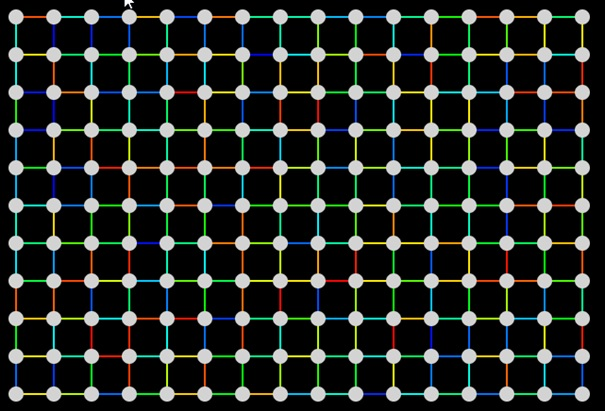
\includegraphics[width=0.5\textwidth]{grafik.jpg}
\caption{\label{fig:graf}Graficzna reprezentacja przykładowego grafu. (Źródło: materiały z ISOD)}
\end{figure}

\paragraph{Program działa w czterech trybach, które należy podać jako pierwszy argument wywołania programu:}
\begin{enumerate}
\item Tryb wczytywania (argument wywołania: \texttt{loadMode})
Program sprawdzi poprawność argumentów i poda wynik w postaci najkrótszej ścieżki i diagramu przejść do pliku tekstowego o określonej nazwie.
W trybie wczytywania użytkownik powinien podać ścieżkę do pliku, na podstawie którego będzie badał, czy istnieje ścieżka pomiędzy dwoma punktami. Następnie podać maksymalnie 10 par punktów. Program znajdzie najkrótszą drogę dla poszczególnych par punktów oraz sprawdzi, czy podany graf jest spójny.

Przykładowe użycie programu 07.03.2022 o godzinie 18:58 z następującymi argumentami:

\texttt{./a.out loadMode mygraph 0 1 1 0 1 6}

Poskutkuje stworzeniem pliku tekstowego mygraph07-03-22-18:58 z następującą zawartością: \\

\texttt{Graf jest spójny\\
Najkrótsza ścieżka od 0 do 1 wynosi 0.8845274871\\
Diagram przejść: 0 - (0.8845274871) - 1 \\
Najkrótsza ścieżka od 1 do 0 wynosi 0.461284698213\\
Diagram przejść: 1 - (0.461284698213) - 0\\
Najkrótsza ścieżka od 0 do 1 wynosi 0.6662378921\\
Diagram przejść: 1 - (0.2643829481) - 5 - (0.4016112941) - 6}

\item Tryb losowy (argument wywołania: \texttt{allRandMode})
Program sprawdzi poprawność argumentów, następnie wygeneruje graf do określonego pliku, a następnie zadziała tak jak w trybie wczytywania.

Dostępne flagi (dla trybów 2., 3., 4.): \\
\texttt{-r   <int> - określ liczbę wierszy grafu (domyślnie 10)\\
-c  <int>  określ liczbę kolumn grafu (domyślnie 10)\\
-low <double> określ dolny przedział przy losowaniu wag (domyślnie 0)\\
-high <double> określ górny przedział przy losowaniu wag (domyślnie 1)\\
-dec <int> określ ilość miejsc  po przecinku (domyślnie 10, maksymalnie 20)\\
-p <int>  <int>,<int>  <int>,<int> …  podaj ilość par punktów , dla których będą szukane ścieżki (domyślnie zostanie wylosowane 5 par)}


Po wywołaniu programu z następującymi parametrami:

\texttt{./a.out allRandMode -c  7 -r 4 -dec 16 –p 3 0 1 1 0 1 6}

Zostanie wygenerowany graf o liczbie wierszy 7, liczbie kolumn 4, z wagami z zakresu od 0 do 1 z dokładnością do 16 miejsc po przecinku (niekoniecznie spójny). Następnie na podstawie wygenerowanego i zapisanego do pliku grafu (allRandGraph7x4) program zadziała tak, jakby podać wygenerowany graf i pary liczb jako argumenty trybu wczytywania.

\item Tryb losowych wag (argument wywołania: \texttt{randWeightMode})
Program sprawdzi poprawność argumentów, następnie wygeneruje graf do określonego pliku, a następnie zadziała tak jak w trybie wczytywania.
W trybie losowych wag użytkownik powinien podać argumenty takie same jak w trybie losowym. Zostanie wygenerowany graf przypominający kartkę w kratkę.

Po wywołaniu programu z następującymi parametrami:

\texttt{./a.out randWeightMode -c  7 -r 4 -dec 16 –p 3 0 1 1 0 1 6}

Zostanie wygenerowany graf o liczbie kolumn 7, liczbie wierszy 4, z wagami z zakresu od 0 do 1 z dokładnością do 16 miejsc po przecinku (graf typu „kartka w kratkę”). Następnie na podstawie wygenerowanego i zapisanego do pliku grafu (squareGraph7x4) program zadziała tak, jakby podać wygenerowany graf i pary liczb jako argumenty trybu wczytywania.

\item Tryb spójności (argument wywołania: \texttt{conMode})
Program sprawdzi poprawność argumentów, następnie wygeneruje graf do określonego pliku, a następnie zadziała tak jak w trybie wczytywania.
W trybie spójności użytkownik powinien podać argumenty takie same jak w trybie losowym. Zostanie wygenerowany graf spójny.

Po wywołaniu programu z następującymi parametrami:

\texttt{./a.out conMode -c  7 -r 4 -dec 16 –p 3 0 1 1 0 1 6}

Zostanie wygenerowany graf o liczbie kolumn 7, liczbie wierszy 4, z wagami z zakresu od 0 do 1 z dokładnością do 16 miejsc po przecinku (graf zawsze spójny). Następnie na podstawie wygenerowanego i zapisanego do pliku grafu (constGraph7x4) program zadziała tak, jakby podać wygenerowany graf i pary liczb jako argumenty trybu wczytywania.
\end{enumerate}

\section{Obsługa błędów}
\paragraph{Możliwe błędy przy uruchamianiu programu:}

\begin{itemize}

\item \texttt{Argument nie jest liczbą, lub zawiera się poza określonym zakresem} \\ 
Ten błąd pojawia się, kiedy jeden z argumentów który powinien być liczbą (kolumny, wiersze, dolny zakres wag, górny zakres wag, dokładność, pary punktów)

\item \texttt{Brak określonego trybu} \\
Ten błąd pojawia się, kiedy pierwszy argument wywołania nie pasuje do żadnego z czterech trybów 

\item \texttt{Nie udało się otworzyć pliku} \\
Ten błąd pojawia się, kiedy nie można uzyskać dostępu do pliku z grafem 
\item \texttt{Nie udało się utworzyć pliku} \\
Ten błąd pojawia się, kiedy nie można było stworzyć pliku z wygenerowanym grafem, lub z odpowiedzią 

\item \texttt{Niepoprawna liczba argumentów } \\
Ten błąd pojawia się, kiedy podana zostanie niewystarczająca lub zbyt duża liczba argumentów 

\item \texttt{Punkt nie należy do grafu} \\
Ten błąd pojawia się, kiedy jakiś punkt podany jako argument wywołania wykracza poza zakres grafu, to znaczy jest większy bądź równy iloczynowi podanych kolumn i wierszy

\end{itemize}

\end{document}
